\section{网络层}

网络层是 TCP/IP 协议栈中最核心的一层，负责将分组从源主机通过中间路由器送达目的主机。408 考试中网络层分值占比极高，CIDR 子网划分、IP 分片偏移计算和路由协议对比是必考内容。

\subsection{网络层提供的两种服务}

网络层向上面的传输层提供怎样的服务，存在两种对立的观点：

\begin{mydef}{虚电路与数据报}{vc-datagram}
\begin{tablebox}{虚电路服务 vs 数据报服务}
\centering
\small
\begin{tabular}{|p{2.8cm}|p{4.8cm}|p{4.8cm}|}
\hline
对比维度 & 虚电路（VC）服务 & 数据报（Datagram）服务 \\
\hline
核心思路 & 面向连接，可靠交付 & 无连接，尽最大努力交付 \\
连接的建立 & 必须先建立连接 & 不需要 \\
终点地址 & 仅建立连接时使用 & 每个分组携带完整目的地址 \\
分组转发依据 & 虚电路号（VCI） & 目的 IP 地址 \\
分组顺序 & 按序到达 & 可能乱序 \\
路由选择 & 建立连接时选一次 & 每个分组独立选路 \\
结点故障影响 & 经过该结点的 VC 全失效 & 仅丢失故障结点的分组 \\
代表网络 & ATM、帧中继、X.25 & Internet（IP） \\
\hline
\end{tabular}
\end{tablebox}
\end{mydef}

\begin{attention}
\textbf{408 核心辨析：} 因特网（Internet）采用数据报服务，网络层只提供\textbf{尽最大努力交付}（Best-Effort Delivery），不保证可靠。可靠传输由传输层（TCP）在端系统中实现。这就是「网络层简单化，端系统智能化」的\textbf{端到端原则}（End-to-End Principle）的体现。

408 常考判断题：「网络层提供可靠的端到端通信」——\textbf{错误}，可靠通信由传输层 TCP 保证。
\end{attention}

\subsection{IPv4 地址}

\subsubsection{IP 地址的分类}

\begin{mydef}{IPv4 地址}{ipv4-addr}
IPv4 地址为 32 位二进制数，通常用\textbf{点分十进制}（Dotted Decimal）表示，如 192.168.1.1。每个 IP 地址由\textbf{网络号（net-id）}和\textbf{主机号（host-id）}两部分组成。
\end{mydef}

\begin{conclusion}{分类 IP 地址（Classful Addressing）}{ip-classes}
\begin{tablebox}{IP 地址分类}
\centering
\small
\begin{tabular}{|c|c|c|p{3.2cm}|c|c|}
\hline
类别 & 网络号位数 & 首字节范围 & 网络号范围 & 最大网络数 & 每网最大主机数 \\
\hline
A 类 & 8 位 & 1--126 & 1.0.0.0--126.0.0.0 & $2^7-2=126$ & $2^{24}-2\approx 1677$ 万 \\
B 类 & 16 位 & 128--191 & 128.0.0.0--191.255.0.0 & $2^{14}=16384$ & $2^{16}-2=65534$ \\
C 类 & 24 位 & 192--223 & 192.0.0.0--223.255.255.0 & $2^{21}\approx209$ 万 & $2^8-2=254$ \\
D 类 & — & 224--239 & 组播地址 & — & — \\
E 类 & — & 240--255 & 保留 & — & — \\
\hline
\end{tabular}
\end{tablebox}
\textbf{特殊地址：}
\begin{itemize}
    \item \textbf{全 0}（0.0.0.0）：本网络上的本主机（DHCP 初始状态）。
    \item \textbf{网络号全 0}：本网络上的特定主机。
    \item \textbf{主机号全 0}：网络地址（标识一个网络）。
    \item \textbf{主机号全 1}：该网络的直接广播地址。
    \item \textbf{全 1}（255.255.255.255）：受限广播（本网络广播，不进路由器）。
    \item \textbf{127.x.x.x}：环回地址（Loopback），典型的为 127.0.0.1。
    \item \textbf{10.x.x.x, 172.16--31.x.x, 192.168.x.x}：私有地址（RFC 1918）。
\end{itemize}
\end{conclusion}

\begin{attention}
\textbf{减 2 的原因：} 主机号全 0 为网络地址，主机号全 1 为广播地址，均不能分配给具体主机，因此可用主机数 = $2^n-2$。408 选择题经常在是否需要「减 2」上设置陷阱。
\end{attention}

\subsubsection{子网划分与子网掩码}

\begin{mydef}{子网划分}{subnetting}
在分类 IP 地址的基础上，从主机号中借用若干位作为\textbf{子网号}（subnet-id），形成三级编址结构：
\[
\text{IP 地址} ::= \{\langle\text{网络号}\rangle,\;\langle\text{子网号}\rangle,\;\langle\text{主机号}\rangle\}
\]
这是对分类 IP 地址的改进，能更有效地利用 IP 地址空间。
\end{mydef}

\begin{formula}{子网掩码}{subnet-mask}
子网掩码（Subnet Mask）用于区分 IP 地址中的网络部分和主机部分：
\begin{itemize}
    \item 网络号位 + 子网号位 $\to$ 掩码中对应位为 \textbf{1}。
    \item 主机号位 $\to$ 掩码中对应位为 \textbf{0}。
\end{itemize}
\[
\text{网络地址} = \text{IP 地址} \;\&\; \text{子网掩码} \quad \text{（按位 AND）}
\]
\textbf{子网掩码表示方式：}
\begin{itemize}
    \item 点分十进制：255.255.255.0（等价于 /24）。
    \item CIDR 前缀长度：「/n」表示前 $n$ 位为网络前缀。
\end{itemize}
\end{formula}

\begin{attention}
\textbf{408 高频计算：} 给定一个 IP 地址和子网掩码，要求计算：(1) 网络地址；(2) 广播地址；(3) 该子网可容纳的主机数；(4) 子网中第一个和最后一个可用的 IP 地址。

\textbf{口诀：} 网络地址 = IP \& 掩码（主机位全 0）；广播地址 = 网络地址 + 主机位全 1；可用 IP 范围 = （网络地址 + 1）到（广播地址 - 1）。
\end{attention}

\subsubsection{CIDR 与路由聚合}

\begin{mydef}{无分类编址 CIDR}{cidr}
CIDR（Classless Inter-Domain Routing，无分类域间路由）彻底消除了传统的 A/B/C 类地址和子网划分的概念，使用\textbf{网络前缀}（Network Prefix）代替网络号：
\[
\text{IP 地址} ::= \{\langle\text{网络前缀}\rangle,\;\langle\text{主机号}\rangle\}
\]
记作 \textbf{IP 地址/前缀长度}，如 192.168.1.0/24。
\end{mydef}

\begin{conclusion}{CIDR 路由聚合（Route Aggregation）}{route-aggregation}
CIDR 的核心优势是\textbf{路由聚合}（构成超网）：将多个连续的子网合并为一个更大的地址块，从而压缩路由表。

\textbf{聚合方法：} 将多个网络地址按位对齐，找出最长的共同前缀。
\[
\text{例如：} 192.168.0.0/24,\; 192.168.1.0/24,\; 192.168.2.0/24,\; 192.168.3.0/24
\]
四个网络地址的前 22 位相同（192.168 的前两个字节 + 第三字节的前 6 位），可聚合为 \textbf{192.168.0.0/22}。

\begin{tablebox}{最长前缀匹配示例}
\centering
\begin{tabular}{|l|l|}
\hline
路由表项 & 下一跳 \\
\hline
192.168.0.0/22 & R1（聚合路由） \\
192.168.2.0/24 & R2（更具体的路由） \\
\hline
\end{tabular}
\end{tablebox}

当目的地址 192.168.2.5 同时匹配两条路由时，路由器选择前缀最长的（/24 > /22）即 R2，这称为\textbf{最长前缀匹配}（Longest Prefix Match）。
\end{conclusion}

\begin{attention}
\textbf{408 必考：CIDR 地址块的计算。} 给定 /n 前缀，则：
\begin{itemize}
    \item 地址块大小 = $2^{32-n}$ 个地址。
    \item 可用地址数 = $2^{32-n} - 2$（去掉全 0 和全 1）。
    \item 地址掩码：前 $n$ 位为 1，后 $32-n$ 位为 0。
    \item 最小地址 = 网络地址（主机位全 0），最大地址 = 广播地址（主机位全 1）。
\end{itemize}
\textbf{路由聚合}（构成超网）是 CIDR 的核心考点，要求从若干连续子网中提取最长公共前缀。
\end{attention}

\subsection{ARP、DHCP 与 ICMP}

\subsubsection{ARP（地址解析协议）}

\begin{mydef}{ARP}{arp}
ARP（Address Resolution Protocol）将 IP 地址映射为 MAC 地址，工作在网络层和数据链路层之间。每台主机维护一个\textbf{ARP 高速缓存}（ARP Cache），存储最近解析的 IP-MAC 映射。
\end{mydef}

\begin{conclusion}{ARP 工作过程}{arp-process}
\begin{enumerate}
    \item 主机 A 要发送数据给同一局域网内的主机 B（已知 B 的 IP，未知 B 的 MAC）。
    \item A 在局域网内\textbf{广播} ARP 请求分组：「谁有 IP 地址 xxx？请告诉我你的 MAC 地址。」
    \item 主机 B 收到后，向 A \textbf{单播} ARP 响应分组：「我的 IP 是 xxx，MAC 地址是 yyy。」
    \item A 将映射关系存入 ARP 缓存，然后用获得到的 MAC 地址封装帧并发送数据。
\end{enumerate}

\textbf{ARP 的四种典型场景：}
\begin{itemize}
    \item 发送方是主机，目的主机在同一网络 $\to$ ARP 解析目的主机的 MAC。
    \item 发送方是主机，目的主机在另一网络 $\to$ ARP 解析默认网关（路由器）的 MAC。
    \item 发送方是路由器，转发到目的主机在同一网络 $\to$ ARP 解析目的主机的 MAC。
    \item 发送方是路由器，转发到下一跳路由器 $\to$ ARP 解析下一跳路由器的 MAC。
\end{itemize}
\end{conclusion}

\begin{attention}
\textbf{408 辨析：} ARP 解决的是同一局域网内的 IP→MAC 映射问题。跨网段通信时，ARP 解析的是\textbf{默认网关的 MAC 地址}，而非目的主机的 MAC 地址。ARP 请求是广播帧（目的 MAC 为 FF-FF-FF-FF-FF-FF），ARP 响应是单播帧。
\end{attention}

\subsubsection{DHCP（动态主机配置协议）}

\begin{mydef}{DHCP}{dhcp}
DHCP（Dynamic Host Configuration Protocol）允许主机自动获取 IP 地址、子网掩码、默认网关和 DNS 服务器地址。基于 UDP，服务器端口 67，客户端端口 68。DHCP 工作在\textbf{应用层}（使用 UDP），但其功能服务于网络层的 IP 地址配置。
\end{mydef}

\begin{conclusion}{DHCP 四步交互（DORA）}{dhcp-dora}
\begin{tablebox}{DHCP 交互过程}
\centering
\begin{tabular}{|c|l|l|l|}
\hline
步骤 & 报文名称 & 方向 & 关键信息 \\
\hline
1 & DHCP DISCOVER & 客户端 $\to$ 服务器（广播） & 客户端寻找 DHCP 服务器 \\
2 & DHCP OFFER & 服务器 $\to$ 客户端 & 服务器提供 IP 地址 \\
3 & DHCP REQUEST & 客户端 $\to$ 服务器（广播） & 客户端请求使用该 IP \\
4 & DHCP ACK & 服务器 $\to$ 客户端 & 服务器确认，租约生效 \\
\hline
\end{tabular}
\end{tablebox}
\textbf{408 常考：} (1) DHCP DISCOVER 和 DHCP REQUEST 都是广播（客户端此时尚无 IP 或尚未确认使用某 IP）；(2) DHCP 租约（Lease）有期限，到期前需续约；(3) DHCP 分配的不仅是 IP 地址，还有子网掩码、默认网关等。
\end{conclusion}

\subsubsection{ICMP（互联网控制报文协议）}

\begin{mydef}{ICMP}{icmp}
ICMP（Internet Control Message Protocol）用于在 IP 主机和路由器之间传递差错报告和控制信息，是 IP 层的配套协议。ICMP 报文封装在 IP 数据报中传输（协议号 = 1）。
\end{mydef}

\begin{conclusion}{ICMP 报文类型与典型应用}{icmp-types}
\begin{tablebox}{常见 ICMP 报文类型}
\centering
\begin{tabular}{|l|c|c|}
\hline
ICMP 报文类型 & 类型值 & 说明 \\
\hline
\textbf{回送请求}（Echo Request） & 8 & Ping 发送的报文 \\
\textbf{回送回答}（Echo Reply） & 0 & Ping 收到的响应 \\
\textbf{终点不可达}（Dest. Unreachable） & 3 & 网络/主机/协议/端口不可达 \\
\textbf{源点抑制}（Source Quench） & 4 & 拥塞控制（已废弃） \\
\textbf{重定向}（Redirect） & 5 & 通知主机使用更好的路由 \\
\textbf{超时}（Time Exceeded） & 11 & TTL 减到 0，Traceroute 使用 \\
\hline
\end{tabular}
\end{tablebox}

\textbf{Ping 的原理：}
\begin{itemize}
    \item 源主机向目的主机发送 ICMP 回送请求（Echo Request，类型 8）。
    \item 目的主机收到后返回 ICMP 回送回答（Echo Reply，类型 0）。
    \item 通过 RTT（往返时间）和丢包率判断网络连通性。
    \item Ping 工作在网络层，不涉及传输层端口。
\end{itemize}

\textbf{Traceroute（Tracert）的原理：}
\begin{itemize}
    \item 源主机依次发送 TTL = 1, 2, 3, ... 的 UDP 数据报（或 ICMP 回送请求）。
    \item 第 $i$ 跳路由器收到 TTL = 0 的数据报后，丢弃并向源主机返回\textbf{ICMP 超时}（类型 11）报文。
    \item 源主机从超时报文的源 IP 地址获知第 $i$ 跳路由器的 IP。
    \item 最终到达目的主机时，目的主机返回 ICMP 终点不可达（端口不可达）报文（因为使用了不可达的 UDP 端口），Traceroute 停止。
\end{itemize}
\end{conclusion}

\begin{attention}
\textbf{408 辨析：}
\begin{itemize}
    \item Ping 使用 ICMP，不经过传输层；它测试的是网络层的连通性。
    \item Traceroute 利用 TTL 字段逐跳发现路径，TTL 减到 0 时路由器返回 ICMP 超时报文。
    \item ICMP 终点不可达报文还可携带差错代码区分「网络不可达」「主机不可达」「协议不可达」「端口不可达」等。
\end{itemize}
\end{attention}

\subsection{IP 数据报格式}

\begin{mydef}{IP 数据报}{ip-datagram}
IP 数据报由\textbf{首部}（Header）和\textbf{数据}（Data/Payload）两部分组成。IPv4 首部固定部分为 20 字节（不含选项字段），最大长度为 60 字节（含选项）。
\end{mydef}

\begin{conclusion}{IPv4 首部字段详解}{ipv4-header}
\begin{tablebox}{IPv4 首部格式（固定部分 20 字节）}
\centering
\begin{tabular}{|l|c|p{7cm}|}
\hline
字段 & 位数 & 说明 \\
\hline
\textbf{版本}（Version） & 4 & 协议版本号，IPv4 = 4 \\
\textbf{首部长度}（IHL） & 4 & 以 4 字节为单位，最小值 5（20 字节），最大值 15（60 字节） \\
\textbf{区分服务}（DS） & 8 & 服务质量（QoS），很少使用 \\
\textbf{总长度}（Total Length）& 16 & 首部 + 数据的总字节数，最大 65535 字节 \\
\textbf{标识}（Identification） & 16 & 标识同一数据报的所有分片 \\
\textbf{标志}（Flags） & 3 & DF（不分片）、MF（还有分片） \\
\textbf{片偏移}（Fragment Offset）& 13 & 本分片在原数据报中的相对位置，以 8 字节为单位 \\
\textbf{生存时间}（TTL） & 8 & 经过的最大跳数，每经一个路由器减 1，减到 0 则丢弃 \\
\textbf{协议}（Protocol） & 8 & 上层协议：TCP=6，UDP=17，ICMP=1，OSPF=89 \\
\textbf{首部校验和}（Header Checksum）& 16 & 仅校验首部，每跳重新计算（TTL 变化） \\
\textbf{源 IP 地址} & 32 & 发送方 IP 地址 \\
\textbf{目的 IP 地址} & 32 & 接收方 IP 地址 \\
\hline
\end{tabular}
\end{tablebox}

\textbf{关键字段说明：}
\begin{itemize}
    \item \textbf{总长度}：最大 65535 字节，但实际受数据链路层 MTU 限制（以太网为 1500 字节）。
    \item \textbf{TTL}：防止数据报在网络中无限循环。每经过一个路由器减 1，减到 0 时丢弃并返回 ICMP 超时报文。Linux 默认 TTL = 64，Windows 默认 TTL = 128。
    \item \textbf{协议}：标识上层协议，使目的主机的 IP 层知道将数据部分交给哪个上层协议处理（类似于传输层端口号的复用/分用功能）。
    \item \textbf{首部校验和}：每经过一个路由器都需重新计算（因为 TTL 字段改变了）。采用反码求和（Internet Checksum），只校验首部不校验数据。
\end{itemize}
\end{conclusion}

\begin{attention}
\textbf{408 常考细节：}
\begin{itemize}
    \item 首部长度字段以 4 字节为单位：值为 5 表示 20 字节，值为 15 表示 60 字节。
    \item 总长度以 1 字节为单位，最大 65535。
    \item 片偏移以 8 字节为单位（乘以 8 得到实际字节偏移量）。
    \item 首部校验和\textbf{每跳重新计算}的原因：TTL 字段每跳变化。
    \item 区分 IP 数据报上层协议：IPv4 用协议字段（Protocol），IPv6 用「下一个首部」（Next Header）。
\end{itemize}
\end{attention}

\subsection{IP 分片与重组}

\begin{mydef}{IP 分片}{ip-fragmentation}
当 IP 数据报长度超过数据链路层的 MTU（Maximum Transmission Unit，最大传输单元）时，路由器将数据报分割为若干更小的\textbf{分片}（Fragment），分别发送。分片可以在源主机和中间路由器进行，但\textbf{重组只在目的主机进行}。
\end{mydef}

\begin{conclusion}{分片相关字段}{frag-fields}
三个字段协同完成分片与重组：
\begin{itemize}
    \item \textbf{标识（Identification，16 位）：} 同一数据报的所有分片具有相同的标识值。目的主机根据标识将分片归组。
    \item \textbf{标志（Flags，3 位）：}
    \begin{itemize}
        \item 第 0 位：保留，必须为 0。
        \item 第 1 位：\textbf{DF（Don't Fragment）}——1 表示禁止分片。若数据报超过 MTU 且 DF=1，路由器丢弃该数据报并返回 ICMP 差错报文。
        \item 第 2 位：\textbf{MF（More Fragments）}——1 表示后面还有分片，0 表示这是最后一个分片。
    \end{itemize}
    \item \textbf{片偏移（Fragment Offset，13 位）：} 本分片的数据部分在原数据报数据部分中的相对位置，\textbf{以 8 字节为单位}。即：实际字节偏移量 = 片偏移值 $\times$ 8。
\end{itemize}
\end{conclusion}

\begin{formula}{分片计算的完整步骤}{frag-calc}
设原数据报数据部分长度为 $L$ 字节，MTU = $M$ 字节，IP 首部固定 20 字节。

\textbf{Step 1：}每个分片可承载的最大数据量 = $M - 20$（取 8 的整数倍，记为 $D_{\text{max}}$）。
\[
D_{\text{max}} = \left\lfloor \frac{M - 20}{8} \right\rfloor \times 8
\]

\textbf{Step 2：}计算分片数量 $n$：
\[
n = \left\lceil \frac{L}{D_{\text{max}}} \right\rceil
\]

\textbf{Step 3：}计算每个分片的：
\begin{itemize}
    \item 数据长度（前 $n-1$ 个分片均为 $D_{\text{max}}$，最后一个为剩余）。
    \item 总长度 = 数据长度 + 20（首部）。
    \item 片偏移 = 前面所有分片数据长度之和 / 8。
    \item MF 标志：除最后一个分片 MF = 0 外，其余 MF = 1（DF 均为 0）。
\end{itemize}
\end{formula}

\begin{attention}
\textbf{408 必考——分片计算的核心陷阱：}
\begin{itemize}
    \item \textbf{片偏移以 8 字节为单位，}而非以字节为单位！片偏移值 $\times$ 8 = 实际字节偏移。
    \item 除最后一个分片外，每个分片的数据部分长度\textbf{必须是 8 的整数倍}（因为片偏移以 8 字节为单位）。
    \item 每个分片都携带完整的 IP 首部（20 字节），所以总长度 = 20 + 数据部分长度。
    \item 分片在源主机或路由器发生，\textbf{重组仅在目的主机进行。}中间路由器不重组分片。
    \item 若某个分片丢失，目的主机丢弃所有已收到的该数据报的分片（不完整的重组）。
\end{itemize}
\end{attention}

\boxed{\textbf{例}} 一个数据报数据部分长度为 3800 字节，经过 MTU = 1420 字节的链路（IP 首部固定 20 字节）。求分片情况。

\textbf{解：}
\[
D_{\text{max}} = \left\lfloor \frac{1420 - 20}{8} \right\rfloor \times 8 = \left\lfloor \frac{1400}{8} \right\rfloor \times 8 = 175 \times 8 = 1400
\]
分片数 $n = \lceil 3800 / 1400 \rceil = \lceil 2.714 \rceil = 3$。

\begin{tablebox}{分片结果}
\centering
\begin{tabular}{|c|c|c|c|c|}
\hline
分片 & 数据长度 & 总长度 & 片偏移值 & MF \\
\hline
1 & 1400 & 1420 & $0/8 = 0$ & 1 \\
2 & 1400 & 1420 & $1400/8 = 175$ & 1 \\
3 & 1000 & 1020 & $2800/8 = 350$ & 0 \\
\hline
\end{tabular}
\end{tablebox}

\subsection{路由算法与路由协议}

\begin{mydef}{路由与路由表}{routing}
路由（Routing）是指为数据报选择从源到目的地的路径。路由器根据\textbf{路由表}（Routing Table）进行转发决策。路由表至少包含两项信息：\textbf{目的网络地址}和\textbf{下一跳地址}。（也可能包含子网掩码、接口、度量值等。）
\end{mydef}

路由协议分为两大类：
\begin{itemize}
    \item \textbf{内部网关协议 IGP}（Interior Gateway Protocol）：在同一个自治系统（AS）内部运行。如 RIP、OSPF。
    \item \textbf{外部网关协议 EGP}（Exterior Gateway Protocol）：在不同 AS 之间运行。如 BGP-4。
\end{itemize}

\textbf{自治系统（AS，Autonomous System）：} 由同一机构管理、使用统一路由策略的一组网络。每个 AS 分配一个全球唯一的 AS 号（ASN）。

\subsubsection{RIP（路由信息协议）}

\begin{mydef}{RIP}{rip}
RIP（Routing Information Protocol）是基于\textbf{距离向量}（Distance Vector）算法的 IGP。使用\textbf{跳数}（Hop Count）作为度量标准，最大跳数为 15（跳数 = 16 表示不可达）。RIP 适用于小型网络。
\end{mydef}

\begin{conclusion}{RIP 的工作原理}{rip-working}
\textbf{距离向量算法（Bellman-Ford 分布式版本）：}
\begin{enumerate}
    \item 每个路由器周期性地（默认 30 秒）向所有邻居发送自己的\textbf{完整路由表}。
    \item 收到邻居的路由表后，路由器检查每一条路由：
    \begin{itemize}
        \item 若目的网络不在自己路由表中 $\to$ 添加该路由，度量值 = 邻居的度量值 + 1。
        \item 若目的网络已存在，且下一跳是同一邻居 $\to$ 更新度量值。
        \item 若目的网络已存在，下一跳不同，且邻居提供的度量值 + 1 < 当前度量值 $\to$ 更新路由。
        \item 否则 $\to$ 保持不变。
    \end{itemize}
    \item 若 180 秒未收到某邻居的路由更新，则标记该邻居为不可达。
\end{enumerate}

\textbf{RIP 的核心问题：}
\begin{itemize}
    \item \textbf{慢收敛（Slow Convergence）：} 好消息传得快，坏消息传得慢（计数到无穷问题）。
    \item \textbf{计数到无穷（Count-to-Infinity）：} 链路故障后，路由器不断将度量值递增，直到 16（无穷大）。
    \item \textbf{解决方法：} 水平分割（Split Horizon）、毒性逆转（Poison Reverse）、触发更新（Triggered Update）。
\end{itemize}
\end{conclusion}

\begin{attention}
\textbf{408 考点：RIP 路由表更新。} 给定初始路由表和收到的邻居路由表，要求用距离向量算法更新路由表。核心规则：
\begin{itemize}
    \item 对邻居发来的每条路由，将其跳数 + 1。
    \item 若目的网络不在本地路由表中，直接加入。
    \item 若目的网络已存在且下一跳相同，无条件更新。
    \item 若目的网络已存在但下一跳不同，比较跳数，取更小的。
    \item RIP 基于 UDP（端口 520），是应用层协议但核心功能是为网络层选路。
\end{itemize}
\end{attention}

\subsubsection{OSPF（开放最短路径优先）}

\begin{mydef}{OSPF}{ospf}
OSPF（Open Shortest Path First）是基于\textbf{链路状态}（Link State）算法的 IGP。使用 Dijkstra 最短路径算法，度量值为链路开销（Cost），通常与带宽成反比（Cost = 参考带宽 / 链路带宽）。OSPF 适用于大型网络。
\end{mydef}

\begin{conclusion}{OSPF 的工作原理}{ospf-working}
\textbf{链路状态算法的五个步骤：}
\begin{enumerate}
    \item \textbf{发现邻居：} 每个路由器通过发送 Hello 报文发现相邻路由器。
    \item \textbf{洪泛 LSA：} 每个路由器将自己与邻居的链路状态封装为 LSA（Link State Advertisement），洪泛到整个区域。
    \item \textbf{构建 LSDB：} 每个路由器收集所有 LSA，构建链路状态数据库（LSDB）——全网的完整拓扑图。
    \item \textbf{Dijkstra 计算：} 以自己为根，执行 Dijkstra 最短路径算法，计算出到达每个网络的最短路径。
    \item \textbf{生成路由表：} 根据计算结果生成路由表。
\end{enumerate}

\textbf{OSPF 的关键特性：}
\begin{itemize}
    \item 直接基于 IP（协议号 89），而非 TCP 或 UDP。
    \item 支持区域划分（Area），区域 0 为骨干区域（Backbone Area）。
    \item 支持等价多路径（ECMP，Equal-Cost Multi-Path）负载均衡。
    \item 链路状态变化时才洪泛更新（而非周期性发送完整路由表）。
    \item 支持认证（明文和 MD5）。
\end{itemize}
\end{conclusion}

\subsubsection{RIP 与 OSPF 的对比}

\begin{conclusion}{RIP vs OSPF（408 必考对比）}{rip-ospf-compare}
\begin{tablebox}{RIP 与 OSPF 对比}
\centering
\begin{tabular}{|l|c|c|}
\hline
对比维度 & RIP & OSPF \\
\hline
\textbf{算法类型} & 距离向量（DV） & 链路状态（LS） \\
\textbf{核心算法} & Bellman-Ford（分布式） & Dijkstra（集中式计算） \\
\textbf{度量值} & 跳数 & 链路开销（带宽决定） \\
\textbf{传递的信息} & 完整路由表（给邻居） & LSA（洪泛至整个区域） \\
\textbf{更新方式} & 周期性（30 s） & 触发式（变化时更新） \\
\textbf{网络规模} & 小型（$\le$ 15 跳） & 大型（支持区域分层） \\
\textbf{收敛速度} & 慢（计数到无穷问题） & 快（全网拓扑一致） \\
\textbf{封装协议} & UDP（端口 520） & IP（协议号 89） \\
\textbf{最大度量值} & 15 跳（16 = $\infty$） & 无硬性上限 \\
\hline
\end{tabular}
\end{tablebox}
\end{conclusion}

\begin{attention}
\textbf{408 辨析：}
\begin{itemize}
    \item RIP 的路由器只知道邻居和到各网络的距离（跳数），不知道全网拓扑。
    \item OSPF 的路由器拥有完整的全网拓扑（LSDB），独立计算最短路径树。
    \item RIP 传递路由表；OSPF 传递链路状态信息（LSA）。
    \item 「RIP 是应用层协议，OSPF 是网络层协议」——408 常见判断题：RIP 基于 UDP 在应用层实现，但核心功能是路由选择；OSPF 直接封装在 IP 数据报中。
\end{itemize}
\end{attention}

\subsubsection{BGP（边界网关协议）}

\begin{mydef}{BGP}{bgp}
BGP（Border Gateway Protocol）是 AS 之间的路由协议，目前版本为 BGP-4。BGP 采用\textbf{路径向量}（Path Vector）算法，基于策略而非纯技术指标选择路由。BGP 是 Internet 的「粘合剂」，连接全球数十万个 AS。
\end{mydef}

\begin{conclusion}{BGP 的工作原理}{bgp-working}
\textbf{路径向量算法的核心：}
\begin{itemize}
    \item 每个 BGP 路由器向邻居（eBGP）或 AS 内其他 BGP 路由器（iBGP）通告自己所知道的\textbf{到达各网络前缀的完整 AS 路径}。
    \item 路由选择综合考虑 AS 路径长度、本地偏好（Local Preference）、MED 等多个属性。
    \item AS 路径中包含的 AS 号用于\textbf{环路检测}：若路由器在收到的路径中发现了自己的 AS 号，则拒绝该路由（避免 AS 级环路）。
\end{itemize}

\textbf{BGP 的特点：}
\begin{itemize}
    \item 基于 TCP（端口 179），可靠传输路由更新。
    \item 发送增量更新（只发送变化的部分），非周期性发送完整路由表。
    \item 是一种\textbf{策略驱动}的路由协议：允许 AS 管理员实施商业关系策略（对等、转接、客户等）。
    \item 对等连接（Peering）不传递，转接（Transit）传递。
\end{itemize}
\end{conclusion}

\begin{attention}
\textbf{408 三层路由对比：}
\begin{itemize}
    \item \textbf{RIP：} 距离向量，跳数，UDP 520，AS 内部，小型。
    \item \textbf{OSPF：} 链路状态，开销，IP 协议 89，AS 内部，大型（分层）。
    \item \textbf{BGP：} 路径向量，策略，TCP 179，AS 之间，全球 Internet。
\end{itemize}
\textbf{「BGP 属于距离向量协议」——错误。} BGP 是路径向量（Path Vector），区别于 RIP 的距离向量（Distance Vector），因为 BGP 传递的是完整 AS 路径而非单纯的距离值。
\end{attention}

\subsection{IPv6}

\begin{mydef}{IPv6}{ipv6}
IPv6 地址为 128 位，用冒号十六进制表示（Colon Hexadecimal），如 \texttt{2001:0db8:0000:0000:0000:ff00:0042:8329}。可省略前导零，连续的零块可用「::」压缩一次。
\end{mydef}

\begin{conclusion}{IPv6 与 IPv4 的主要差异}{ipv6-vs-ipv4}
\begin{tablebox}{IPv4 vs IPv6 对比}
\centering
\begin{tabular}{|l|c|c|}
\hline
对比维度 & IPv4 & IPv6 \\
\hline
地址长度 & 32 位 & 128 位 \\
地址表示 & 点分十进制 & 冒号十六进制 \\
首部长度 & 可变（20--60 字节） & 固定 40 字节（基本首部） \\
首部校验和 & 有（每跳重算） & 无（由上层保证） \\
分片 & 源和中间路由器均可分片 & 仅源结点可分片 \\
选项 & 在首部中（IHL 字段处理） & 扩展首部（Next Header 链） \\
协议字段 & Protocol & Next Header \\
ARP & 有（广播 ARP 请求） & 用 NDP（ICMPv6 多播）取代 \\
广播 & 有 & 无（改用多播和任播） \\
NAT & 广泛使用 & 原则上不需要 \\
\hline
\end{tabular}
\end{tablebox}

\textbf{IPv6 基本首部（固定 40 字节）的八个字段：}
版本（4 位）、通信量类（8 位）、流标号（20 位）、有效载荷长度（16 位）、下一个首部（8 位）、跳数限制（8 位）、源地址（128 位）、目的地址（128 位）。

\textbf{从 IPv4 向 IPv6 过渡的技术：}
\begin{itemize}
    \item \textbf{双协议栈（Dual Stack）：} 主机/路由器同时运行 IPv4 和 IPv6。
    \item \textbf{隧道技术（Tunneling）：} IPv6 数据报封装在 IPv4 数据报中穿过 IPv4 网络。
    \item \textbf{协议转换/NAT64：} 在 IPv4-only 和 IPv6-only 网络之间转换。
\end{itemize}
\end{conclusion}

\begin{attention}
\textbf{408 常考细节：}
\begin{itemize}
    \item IPv6 基本首部固定 40 字节（vs IPv4 最小 20 字节）。
    \item IPv6 没有首部校验和字段（因为数据链路层和上层协议已有差错检测）。
    \item IPv6 中间路由器\textbf{不分片}，分片仅在源结点进行。若路径 MTU 不够，路由器丢弃并返回 ICMPv6「分组太大」报文。
    \item IPv6 用 NDP（邻居发现协议，ICMPv6 的一部分）取代 IPv4 中的 ARP。
    \item IPv6 地址类型：单播（Unicast）、多播（Multicast）、任播（Anycast）。无广播。
\end{itemize}
\end{attention}

\subsection{IP 组播与移动 IP}

\subsubsection{IP 组播}

\begin{mydef}{IP 组播}{ip-multicast}
IP 组播（Multicast）实现一对多通信：源主机发送一份数据，由网络负责复制并发送给组播组中的所有成员。组播地址范围：224.0.0.0/4（D 类地址 224.0.0.0--239.255.255.255）。
\end{mydef}

\begin{conclusion}{组播的核心概念}{multicast-concepts}
\begin{itemize}
    \item \textbf{组播组（Multicast Group）：} 用 D 类 IP 地址标识，主机通过 IGMP 协议加入/离开组播组。
    \item \textbf{IGMP（Internet 组管理协议）：} 运行在主机和本地组播路由器之间，用于管理组成员关系。
    \item \textbf{组播路由协议：} 如 PIM（Protocol Independent Multicast），根据组成员分布构建组播分发树。
    \item \textbf{组播 MAC 地址：} 以太网中，组播 IP 到组播 MAC 有固定映射：MAC 地址前 25 位为 01-00-5E，后 23 位为组播 IP 的低 23 位。
\end{itemize}

\textbf{408 常考：} (1) 组播地址只能用作目的地址，不能作为源地址；(2) 组播在局域网内不需要 IGMP 也能工作，但跨路由器转发需要组播路由协议；(3) 组播数据报的 TTL 字段用于限制组播范围。
\end{conclusion}

\subsubsection{移动 IP}

\begin{mydef}{移动 IP}{mobile-ip}
移动 IP 允许移动结点在改变网络接入点时保持其 IP 地址不变，从而保持正在进行的 TCP 连接不中断。
\end{mydef}

\begin{conclusion}{移动 IP 的基本概念}{mobile-ip-concepts}
移动 IP 引入三个功能实体：
\begin{itemize}
    \item \textbf{移动结点（MN，Mobile Node）：} 从一个网络移动到另一个网络的主机。
    \item \textbf{归属代理（HA，Home Agent）：} 移动结点「家乡」网络上的路由器，截获发往移动结点家乡地址的数据报并转发到移动结点的当前位置。
    \item \textbf{外地代理（FA，Foreign Agent）：} 移动结点当前所在网络上的路由器，为移动结点提供路由服务（IPv6 中不需要 FA，移动结点可自行配置转交地址）。
\end{itemize}

\textbf{两个关键地址：}
\begin{itemize}
    \item \textbf{家乡地址（Home Address）：} 移动结点在归属网络中使用的永久 IP 地址。
    \item \textbf{转交地址（Care-of Address，CoA）：} 移动结点在外地网络中使用的临时 IP 地址。
\end{itemize}

\textbf{基本工作过程（三角路由）：}
\[
\text{通信对端 } \xrightarrow{\text{数据报发往家乡地址}} \text{ HA } \xrightarrow{\text{隧道封装到 CoA}} \text{ MN } \xrightarrow{\text{直接回复}} \text{通信对端}
\]
从通信对端 $\to$ HA $\to$ MN 的路径形成一个「三角形」，因此称为\textbf{三角路由}（Triangle Routing）。
\end{conclusion}

\begin{attention}
\textbf{408 概念辨析：} 移动 IP 解决的是 IP 地址与网络位置绑定导致的连接中断问题。核心思想：家乡地址是永久标识（身份），转交地址是当前定位。HA 通过隧道（IP-in-IP 封装）将数据报转发给 MN。
\end{attention}

\subsection{408 高频考点速查}

\begin{conclusion}{网络层 — 408 常考点}{cn4-keypoints}
\begin{enumerate}
    \item \textbf{CIDR 子网划分与路由聚合：} 给定地址块 /n，求网络地址、广播地址、可用地址数；给定多个连续子网，求最大聚合前缀。
    \item \textbf{IP 分片计算：} 给定 MTU 和原数据报长度，计算各分片的数据长度、总长度、片偏移值和 MF 标志（注意片偏移以 8 字节为单位）。
    \item \textbf{RIP 距离向量路由表更新：} 给定初始路由表和收到的邻居路由表，更新本地路由表。
    \item \textbf{RIP vs OSPF vs BGP 的三层对比：} 算法类型、度量值、封装协议、应用场景。
    \item \textbf{IP 首部字段：} TTL、Protocol、Header Checksum、Fragment Offset（各字段作用和 408 陷阱）。
    \item \textbf{ARP 的工作范围：} 同一局域网内的 IP→MAC 解析，ARP 请求是广播帧。
    \item \textbf{ICMP 的 Ping 和 Traceroute 原理：} Echo/Echo Reply（Ping）、Time Exceeded（Traceroute）。
    \item \textbf{IPv6 的关键变化：} 128 位地址、无首部校验和、仅源结点分片、NDP 取代 ARP。
    \item \textbf{虚电路 vs 数据报：} Internet 采用数据报（Best-Effort），可靠由传输层 TCP 完成。
\end{enumerate}
\end{conclusion}

\newpage
\section{习题}

\subsection{基础过关题}

\begin{enumerate}

\item \textbf{（单项选择题）} 以下关于 IP 协议的说法，正确的是
\begin{center}
\begin{tabular}{ll}
(A) IP 协议提供可靠的端到端数据传输服务 \\[4pt]
(B) IP 协议的首部校验和字段校验整个 IP 数据报 \\[4pt]
(C) IP 分片可以在路由器上进行，重组只能在目的主机进行 \\[4pt]
(D) IP 协议在传输层之上运行
\end{tabular}
\end{center}

\item \textbf{（单项选择题）} 一个网络的 IP 地址为 192.168.1.0/26，则该网络可分配的主机地址数为
\begin{center}
\begin{tabular}{ll}
(A) 64 & (B) 62 \\[6pt]
(C) 128 & (D) 126
\end{tabular}
\end{center}

\item \textbf{（单项选择题）} ARP 协议的主要功能是
\begin{center}
\begin{tabular}{ll}
(A) 将域名解析为 IP 地址 \\[4pt]
(B) 将 IP 地址解析为 MAC 地址 \\[4pt]
(C) 将 MAC 地址解析为 IP 地址 \\[4pt]
(D) 发现网络中的路由器
\end{tabular}
\end{center}

\item \textbf{（单项选择题）} Traceroute 程序利用 ICMP 的哪种报文来实现路径跟踪？
\begin{center}
\begin{tabular}{ll}
(A) Echo Request（类型 8） \\[4pt]
(B) Echo Reply（类型 0） \\[4pt]
(C) Time Exceeded（类型 11） \\[4pt]
(D) Destination Unreachable（类型 3）
\end{tabular}
\end{center}

\item \textbf{（单项选择题）} 以下关于 RIP 和 OSPF 的说法，\textbf{错误}的是
\begin{center}
\begin{tabular}{ll}
(A) RIP 基于距离向量算法，OSPF 基于链路状态算法 \\[4pt]
(B) RIP 的最大度量值为 15 跳 \\[4pt]
(C) RIP 和 OSPF 都属于内部网关协议（IGP） \\[4pt]
(D) RIP 使用 IP 直接封装，OSPF 使用 UDP 封装
\end{tabular}
\end{center}

\item \textbf{（填空题）} 在 CIDR 地址块 172.16.0.0/20 中，可用的主机地址数为 \underline{\qquad}。若将其划分为 4 个等长子网，每个子网的前缀长度为 \underline{\qquad}。

\item \textbf{（填空题）} IPv4 数据报首部固定部分为 \underline{\qquad} 字节。首部长度字段以 \underline{\qquad} 字节为单位，片偏移字段以 \underline{\qquad} 字节为单位。

\item \textbf{（填空题）} IPv6 地址长度为 \underline{\qquad} 位，基本首部固定为 \underline{\qquad} 字节。IPv6 用 \underline{\qquad} 协议取代了 IPv4 中的 ARP。

\item \textbf{（简答题）} 简述 Ping 程序的工作原理（说明其使用的协议和报文类型）。

\item \textbf{（计算题）} 一个 IP 数据报的数据部分为 4000 字节，经过一条 MTU = 1500 字节的链路（固定首部长度 20 字节）。计算：
\begin{enumerate}
    \item[(1)] 需要分成几个分片？
    \item[(2)] 每个分片的数据长度、总长度、片偏移值和 MF 标志。
\end{enumerate}

\end{enumerate}

\subsection{真题风格与综合训练}

\begin{enumerate}[resume]

\item \textbf{（真题风格，单项选择题）} 某路由器收到一个 IP 数据报，其首部中 TTL 字段的值为 1。以下对该数据报的处理方式，正确的是
\begin{center}
\begin{tabular}{ll}
(A) 正常转发该数据报 \\[4pt]
(B) 将 TTL 减 1 后转发 \\[4pt]
(C) 丢弃该数据报，并向源主机发送 ICMP 超时报文 \\[4pt]
(D) 丢弃该数据报，不发送任何差错报文
\end{tabular}
\end{center}

\item \textbf{（真题风格，单项选择题）} 以下四个子网：
\[
192.168.4.0/24,\quad 192.168.5.0/24,\quad 192.168.6.0/24,\quad 192.168.7.0/24
\]
进行路由聚合后，最合适的聚合地址是
\begin{center}
\begin{tabular}{ll}
(A) 192.168.4.0/22 & (B) 192.168.4.0/23 \\[6pt]
(C) 192.168.0.0/21 & (D) 192.168.4.0/24
\end{tabular}
\end{center}

\item \textbf{（真题风格，综合题）} 某网络拓扑中，路由器 R1 的路由表如下：

\begin{tablebox}{R1 的初始路由表}
\centering
\begin{tabular}{|c|c|c|}
\hline
目的网络 & 距离（跳数） & 下一跳 \\
\hline
N1 & 3 & R2 \\
N2 & 4 & R3 \\
N3 & 2 & R2 \\
N4 & 5 & R3 \\
N5 & 6 & R4 \\
\hline
\end{tabular}
\end{tablebox}

R1 收到邻居 R2 发来的路由更新报文（RIP），R2 的路由表如下：

\begin{tablebox}{R2 的路由表}
\centering
\begin{tabular}{|c|c|}
\hline
目的网络 & 距离（跳数） \\
\hline
N1 & 2 \\
N3 & 3 \\
N5 & 3 \\
N6 & 4 \\
\hline
\end{tabular}
\end{tablebox}

\begin{enumerate}
    \item[(1)] 根据 RIP 距离向量算法，更新 R1 的路由表，写出更新后的完整路由表（含目的网络、距离和下一跳）。
    \item[(2)] 简要说明此更新中，哪些路由发生了变化及其原因。
\end{enumerate}

\item \textbf{（真题风格，综合题）} 某主机 A 的 IP 地址为 192.168.10.66/27，请回答以下问题：
\begin{enumerate}
    \item[(1)] 写出该主机所在子网的子网掩码（点分十进制形式）；
    \item[(2)] 该子网的网络地址和广播地址分别是什么？
    \item[(3)] 该子网最多可容纳多少台主机？第一个可用和最后一个可用的 IP 地址分别是什么？
    \item[(4)] 若该网络被进一步划分为 4 个等长子网，新的子网掩码是什么？每个子网可容纳多少台主机？
\end{enumerate}

\item \textbf{（真题风格，综合题）} 某网络使用 OSPF 作为内部网关协议，拓扑结构如下：

\begin{center}
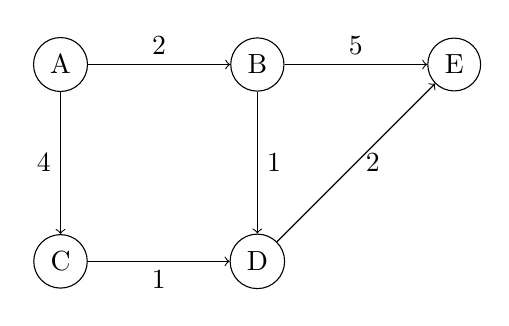
\begin{tikzpicture}[node distance=2.5cm, auto]
\node[draw, circle] (A) {A};
\node[draw, circle, right of=A] (B) {B};
\node[draw, circle, below of=A] (C) {C};
\node[draw, circle, right of=C] (D) {D};
\node[draw, circle, right of=B] (E) {E};

\draw[->] (A) -- node[above] {2} (B);
\draw[->] (A) -- node[left] {4} (C);
\draw[->] (B) -- node[right] {1} (D);
\draw[->] (C) -- node[below] {1} (D);
\draw[->] (B) -- node[above] {5} (E);
\draw[->] (D) -- node[right] {2} (E);
\end{tikzpicture}
\end{center}

图中结点 A--E 代表路由器，边上的数字代表链路开销（Cost）。所有链路均为双向链路。
\begin{enumerate}
    \item[(1)] 以 A 为源结点，使用 Dijkstra 算法计算 A 到所有其他结点的最短路径。写出每一步的结点集合 N 和到达各结点的最短距离。
    \item[(2)] 给出 A 的路由表（目的结点、下一跳、总开销）。
\end{enumerate}

\item \textbf{（真题风格，综合题）} 主机 A 向主机 B 发送一个数据部分长度为 5000 字节的 IP 数据报。A 与 B 之间经过路由器 R1，链路 MTU 如下：A—R1 段 MTU = 1500 字节；R1—B 段 MTU = 600 字节。IP 固定首部均为 20 字节。
\begin{enumerate}
    \item[(1)] 该数据报在 A—R1 段是否需要分片？如需分片，计算各分片的片偏移值、MF 标志和总长度。
    \item[(2)] 分片到达 R1 后，R1 能否在 R1—B 段直接转发？R1 应如何处理？（说明是否需要再次分片及原因。）
    \item[(3)] 最终到达 B 时共有多少个分片？写出每个分片的片偏移值（以 8 字节为单位）。
\end{enumerate}

\item \textbf{（真题风格，简答题）} 请从以下五个维度对比 RIP 和 OSPF 两种内部网关协议：
\begin{enumerate}
    \item[(1)] 路由算法类型及核心思想；
    \item[(2)] 路由度量值；
    \item[(3)] 信息传递方式和范围；
    \item[(4)] 收敛速度及其原因；
    \item[(5)] 适用的网络规模及其原因。
\end{enumerate}

\end{enumerate}

\vspace{8pt}
\noindent\textbf{拓展阅读：}
\begin{itemize}
    \item Kurose \& Ross《计算机网络：自顶向下方法》第 4 章（网络层：数据平面）和第 5 章（网络层：控制平面）——IP 协议详解、CIDR、分片、路由算法（OSPF/BGP）的最权威教材表述。第 4.3 节对路由器内部工作原理的介绍也很精彩。
    \item 谢希仁《计算机网络》第 4 章——网络层体系的国内标准术语（与 408 考纲对齐），特别是 IP 数据报格式的图示和 ICMP 报文格式。
    \item 陈海波《现代操作系统：原理与实现》第 9 章——网络 I/O 和协议栈实现，作为 OS 视角的补充（理解内核如何处理 IP 分片、重组和路由查找）。
    \item RFC 791（IPv4）、RFC 2460（IPv6）、RFC 2453（RIPv2）、RFC 2328（OSPFv2）、RFC 4271（BGP-4）——各协议的标准规范，适合深入查阅细节。
\end{itemize}
